\section{Parallel Logging}
Parallel logging uses multiple loggers and corresponding log files in order to improve the performance of the logging process. While serial logging assumes conflicts between every pair of transactions in the serializable order, parallel logging looks at the "true" dependency. While pairs of transactions with true dependency have to log seqentially, independent transactions should log in parallel. The parallel logging algorithm implements this key observation by explicitly tracking the dependency information between different transactions. In addition, the concurrency control algorithm is implemented to ensure the serializability of the transactions that we have parsed into different threads. \par

% [yxy] One thing you can probably emphasize:
% Serial logging writes logs sequentially, because they assume every 
% pair of transactions may conflict with each other. Ideally, however, 
% we only need transactions with true dependency to log sequentially, 
% while independent transactions should log in parallel. Our parallel 
% logging achieves exactly this, by explicitly tracking the dependency 
% information between different transactions. 

Recall from the serial logging algorithm section that there are four types of dependcies, of which WAW and RAW must be maintained. We argue, however, that WAR dependency, also known as  \textbf{anti-dependency}, does not have to be maintained to preserve the data consistency of the system. To illustrate our claim, we may look at the following example. 
\caption{WAR dependencies}
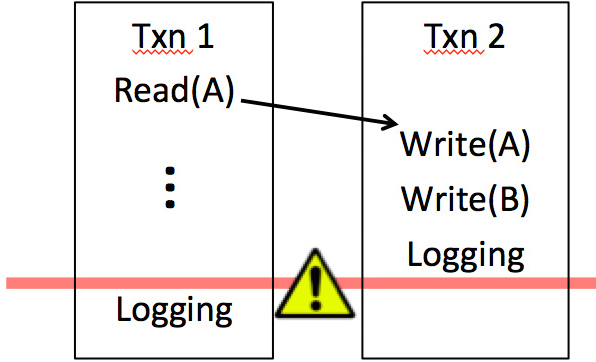
\includegraphics[width=\textwidth]{WAR.jpg}
\end{figure}\\

% [yxy] you may say that the reading transaction does not have any 
% side effect in the database system. So whether it logs or not does 
% not affect the writing transaction.
Even if the system crashes before transaction 1 is logged and after transaction 2 is logged, there will be no conflicts in data consistency during recovery. All the values in the data tuples reflect the exact state of the system immediately before the crash. Transaction 1 does not have any side effect on tuple $A$ in the database system, so whether it logs or not does not affect transaction 2.\par

Note that this will significantly decrease the time complexity of the logging algorithm because the number of writers to a data tuple is significantly smaller than the number of readers. In other words, transaction $A$ depends on the all the transactions executed before $A$ that write to $A$'s data tuples; therefore, $A$ can be logged once all the last writers to its data tuples have been logged. \par

To implement our algorithm, we specify the maximum log sequence number (LSN) in each log file that the transaction currently being logged depends on. When we attempt to log a transaction to the file, we compare the LSN that the transaction depends on ($A$) to the maximum LSN that has already been logged in each file ($B$). If $A\leq B$, the transaction is ready for logging; if $A>B$, we will push the transaction into a waiting queue after arbitrarily assigning it a LSN. The waiting queue will be checked periodically later on to see if any of its contents becomes ready for logging.\par

We use the following example to demonstrate the mechanism of our parallel logging algorithm: 
\begin{figure}[!h]
\caption{Example for Parallel Logging Algorithm and Recovery}
\centering
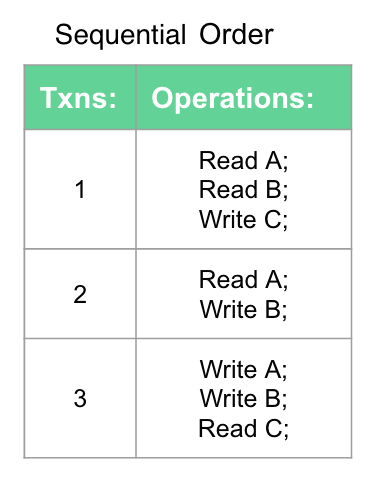
\includegraphics[height=120pt]{Parallel.png}
\hspace{20pt}
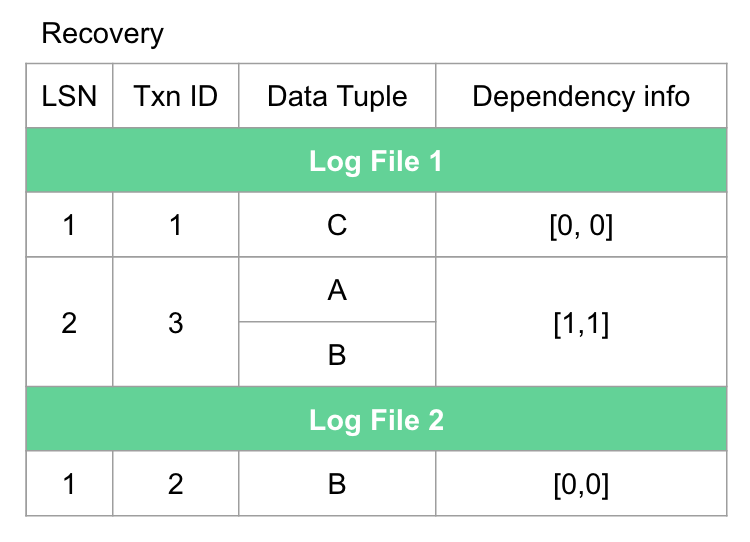
\includegraphics[height=120pt]{Parallel_re.png}
\end{figure}\par
As we mentioned earlier, if we were to use the serial logging algorithm, we would be forced to log the three transactions one by one; when handling big data systems, this can be a serious bottleneck. Meanwhile, the parallel logging algorithm allows us to log multiple transactions with low latency. In this case, note that transactions 1 and 2 can be logged independently since tuple $A$ has no dependency and tuple $B$ is WAR, which, per our discussion above, allows for independent logging. Therefore, if transactions 1 and 2 are parsed into two different threads, they can both be logged without waiting. Transaction 3 depends on transaction 1 due to tuple $C$ (RAW) and on transaction 2 due to tuple $B$ (WAW), so it will be put into the waiting queue until both transaction 1 and 2 have already been logged. 
We follow a similar process during recovery: we read the maximum LSN in each file that the current transaction depends on, and we compare it with the maximum LSN that has been recovered from that file. This ensures the serializability of the log records while improving the efficiency of the recovery process. In this particular example, two different threads take care of the two log files. While transactions 1 and 2 can be recovered immediately, transaction 3 is pushed into the waiting queue until both 1 and 2 have already been recovered.\par
A visualization of the comparison of three log algorithm is below.  